
\chapter{MATERIAIS E MÉTODOS}

Este capítulo descreve a metodologia empregada no desenvolvimento e avaliação do sistema proposto para a detecção automatizada de melanoma. O processo metodológico foi estruturado de modo a refletir o ciclo completo de análise, desde a preparação dos dados e das máscaras de segmentação de referência até a geração do diagnóstico final mediado por agentes baseados em modelos de linguagem natural. A abordagem adotada combina segmentação por \textit{ground truth}, modelos de linguagem multimodal e sistemas multiagentes, com o objetivo de reproduzir, de forma automatizada e explicável, a lógica do raciocínio clínico humano segundo o protocolo ABCD.

\section{Estrutura Geral da Pesquisa}

A Figura~\ref{fig:estrutura_geral} apresenta o fluxo geral da metodologia proposta, que integra técnicas de visão computacional, modelos de linguagem de larga escala (LLMs) e coordenação multiagente para a análise automatizada de lesões cutâneas. O sistema foi projetado de forma modular, permitindo a substituição e o aprimoramento independente de seus componentes, mantendo a coerência entre as etapas de processamento, inferência e validação.

O processo inicia-se na \textbf{Entrada de Dados e Pré-Processamento}, etapa responsável pelo recebimento das imagens de lesões provenientes do conjunto PH2 \cite{mendonca2013ph2}, composto por 200 imagens dermatoscópicas acompanhadas de máscaras de segmentação de referência (\textit{ground truth}, GT) produzidas por especialistas. As imagens são normalizadas e redimensionadas antes de serem encaminhadas ao módulo seguinte. Em substituição a um modelo de segmentação automática, as máscaras GT são utilizadas diretamente como entrada ao sistema, garantindo que a variabilidade introduzida por erros de segmentação não interfira na avaliação do componente de raciocínio das LLMs. Essas máscaras fornecem ao sistema informações estruturais precisas, como área, contorno e assimetria da lesão, essenciais para as etapas posteriores.

Em seguida, a imagem segmentada é encaminhada ao módulo de \textbf{Análise Multiagente}, dividido em duas camadas funcionais. Na \textit{primeira camada}, três agentes especializados,  cada um correspondente a um protocolo diagnóstico clínico distinto (ABCD, Menzies e Seven-Point Checklist),  analisam a lesão de forma independente, gerando diagnósticos preliminares no formato estruturado em JSON. Essa redundância intencional promove diversidade interpretativa e amplia a cobertura diagnóstica, uma vez que cada agente é guiado por heurísticas médicas complementares. Na \textit{segunda camada}, um agente sintetizador (Summary Agent) integra os resultados parciais, produzindo um relatório consolidado que indica o diagnóstico final, sua justificativa e as recomendações clínicas correspondentes.

Como etapa complementar do desenho arquitetural, prevê-se uma \textbf{Validação Acadêmica}, a ser conduzida por um agente crítico fundamentado em \textit{Retrieval-Augmented Generation} (RAG), que consultaria fontes biomédicas de referência (por exemplo, PubMed e literatura de oncologia dermatológica) para verificar a consistência e plausibilidade do diagnóstico proposto. Conforme detalhado na Seção~\ref{sec:avaliacao_experimental}, esse componente permanece em estágio preliminar de implementação e não integrou a versão do sistema avaliada nos experimentos deste trabalho.

Por fim, a \textbf{Saída do Sistema} consolida o diagnóstico validado e o apresenta em linguagem natural ao usuário, juntamente com um prognóstico interpretável e recomendações de acompanhamento. Essa etapa é pensada para futuras aplicações em plataformas de apoio à decisão clínica e teledermatologia, priorizando clareza, auditabilidade e integração com fluxos médicos reais.

\begin{figure}[H]
	\centering
	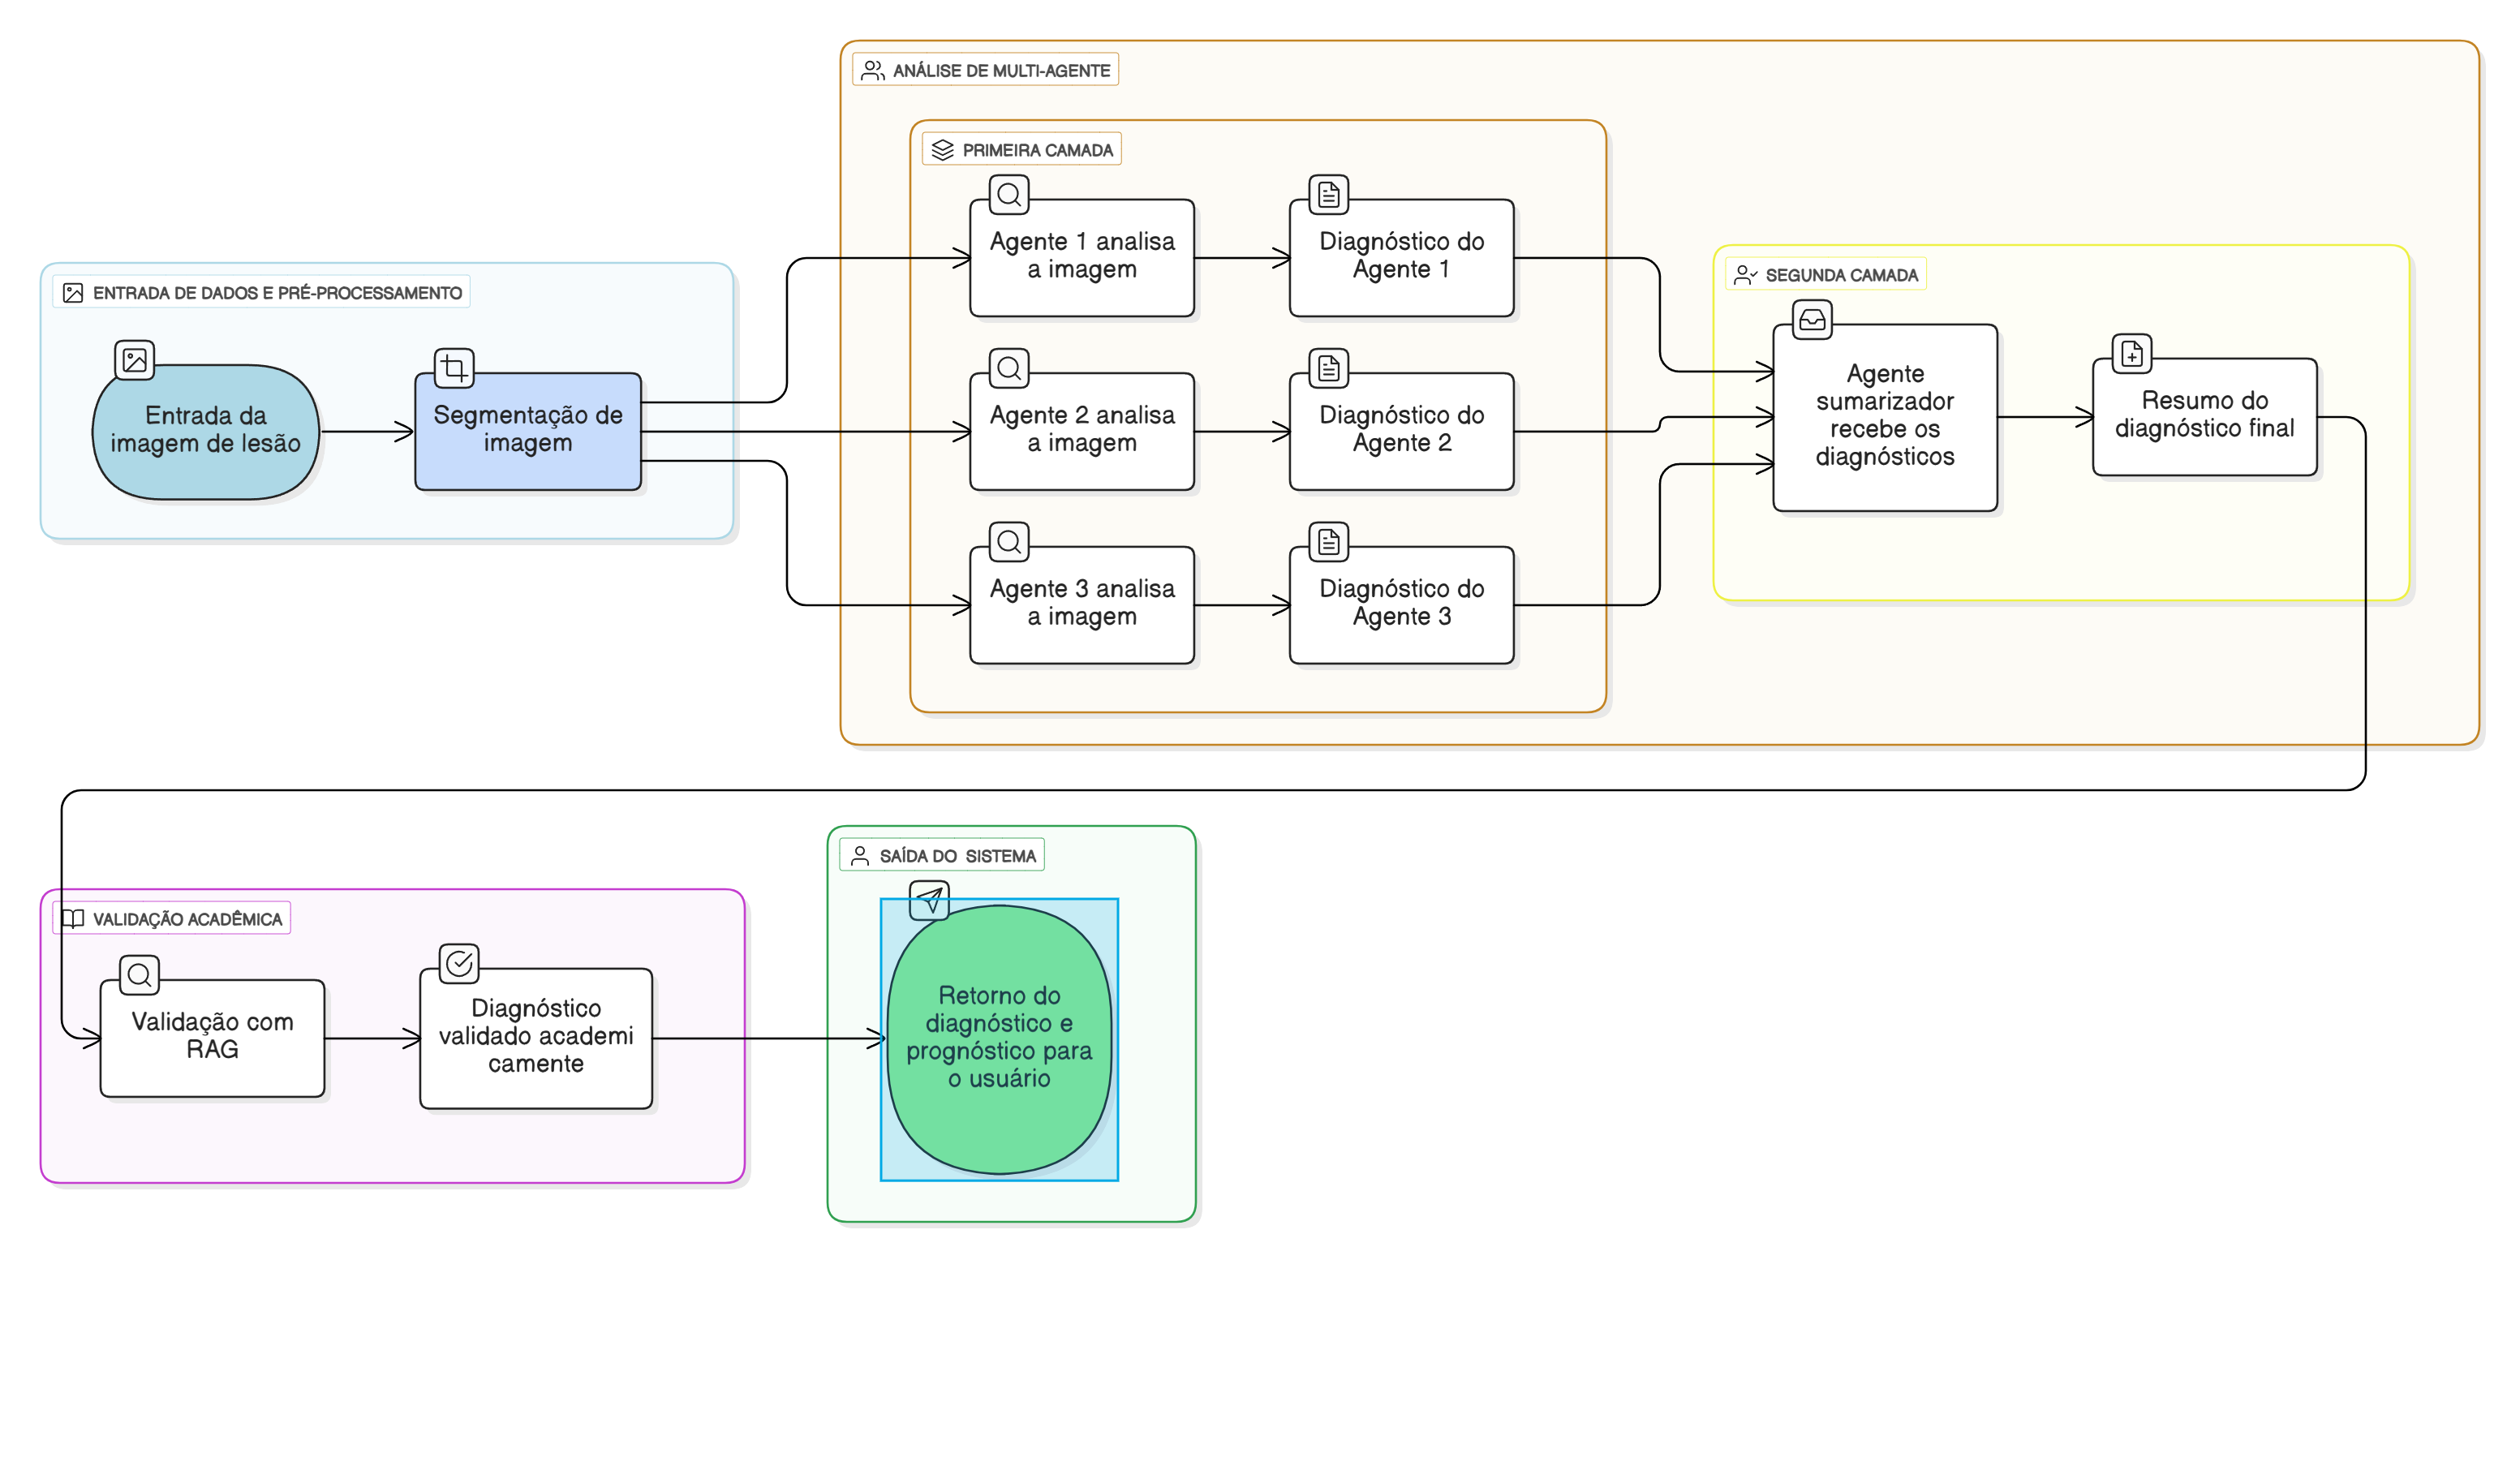
\includegraphics[width=0.95\textwidth]{imagens/Ch3/eraser_diagram.png}
	\caption{Estrutura geral da metodologia proposta, dividida em quatro módulos: (i) entrada e pré-processamento de imagens; (ii) análise multiagente com duas camadas funcionais; (iii) validação acadêmica via RAG, ainda em estágio preliminar de implementação; e (iv) saída interpretável ao usuário.}
	\label{fig:estrutura_geral}
\end{figure}

Dessa forma, a estrutura metodológica reflete um ciclo completo de análise, indo desde a aquisição da imagem até a validação textual baseada em evidências, buscando aproximar o comportamento do sistema de um processo de raciocínio clínico supervisionado e auditável.

\section{Coleta e Pré-processamento dos Dados}
\label{sec:data_preprocessing}

A etapa de coleta e pré-processamento constitui a base empírica desta pesquisa, garantindo a qualidade e a consistência dos dados utilizados para a geração e análise dos diagnósticos pelos agentes. A \autoref{fig:dataflow} apresenta o fluxo geral de integração entre o conjunto de dados PH2, as máscaras de segmentação de referência e o sistema multiagente de diagnóstico proposto.

O conjunto de dados utilizado é o \textbf{PH2} \cite{mendonca2013ph2}, uma base dermoscópica pública composta por 200 imagens digitais adquiridas no Hospital Pedro Hispano (Portugal). Cada imagem é acompanhada de uma máscara binária de segmentação anotada manualmente por especialistas dermatologistas, que delimita com precisão a região da lesão. As imagens são distribuídas em três categorias diagnósticas: 80 nevos comuns, 80 nevos atípicos e 40 melanomas. Para a tarefa de detecção binária adotada neste trabalho, as lesões foram agrupadas em duas classes: \textbf{melanoma} (40 imagens) e \textbf{não-melanoma} (160 imagens, incluindo nevos comuns e atípicos).

O pré-processamento incluiu redimensionamento padronizado das imagens, conversão para o formato aceito pelas APIs dos modelos de linguagem e organização em pares (imagem original, máscara de segmentação de referência) para envio simultâneo aos agentes. Para viabilizar uma avaliação balanceada dos modelos de linguagem, o desequilíbrio original entre as classes (40 melanomas vs.\ 160 não-melanomas, proporção 1:4) foi corrigido por meio de \textit{undersampling}, compondo um subconjunto de teste balanceado com 25 imagens de melanoma e 25 imagens de não-melanoma (50 imagens no total). A seleção das imagens de não-melanoma foi realizada por amostragem aleatória simples, sem estratificação entre nevos comuns e atípicos, com semente fixa (\textit{seed}=42) para garantir reprodutibilidade. Esse subconjunto balanceado foi utilizado na avaliação dos modelos de linguagem GPT-5.4-nano e Gemini-3.1-flash-lite. O \textit{baseline} ResNet-50, por sua vez, foi treinado e avaliado sobre uma divisão treino/teste estratificada distinta do PH2 (Seção~\ref{sec:limitacoes} do Capítulo~5 detalha essa diferença metodológica entre os conjuntos de teste). Cada imagem foi processada em dois formatos: \textbf{imagem original}, que preserva o contexto visual completo, e \textbf{imagem segmentada}, obtida pela aplicação da máscara GT sobre a imagem original. Ambas as versões foram enviadas simultaneamente aos agentes diagnósticos, permitindo análise multimodal e diferentes níveis de foco visual.

\begin{figure}[H]
	\centering
	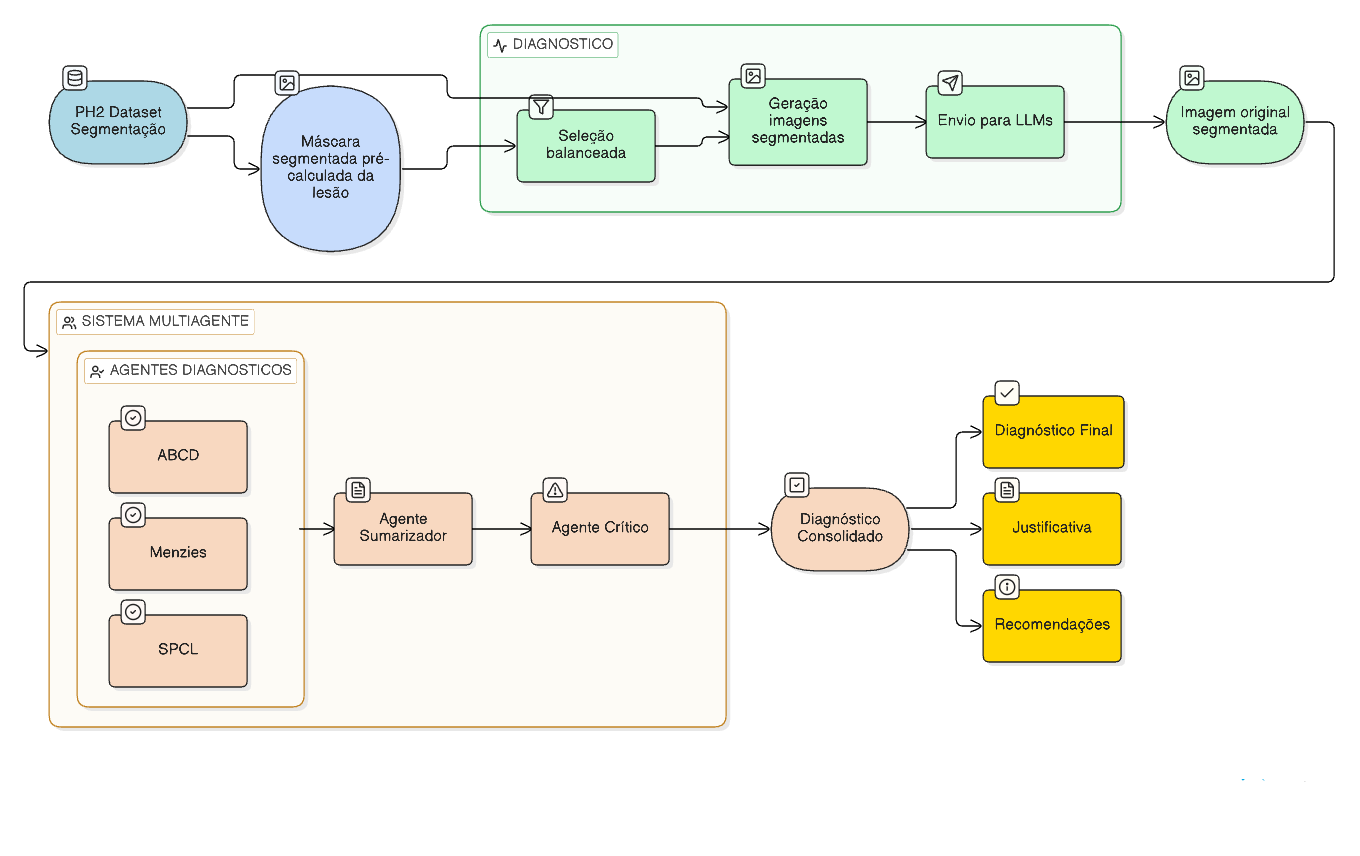
\includegraphics[width=\textwidth]{imagens/Ch3/eraser_data_diagram.png}
	\caption{Fluxo geral de coleta, pré-processamento e integração do conjunto PH2 e suas máscaras de segmentação de referência com o sistema multiagente.}
	\label{fig:dataflow}
\end{figure}



\section{Segmentação: Uso de Máscaras de Referência}

A segmentação das lesões cutâneas constitui uma etapa essencial do \textit{pipeline} diagnóstico, pois fornece ao sistema multiagente uma representação visual delimitada da área de interesse, reduzindo ruídos contextuais e direcionando a atenção dos modelos de linguagem para as características morfológicas da lesão.

Neste trabalho, optou-se por utilizar as \textbf{máscaras de segmentação de referência} (\textit{ground truth} - GT) disponíveis no conjunto PH2, produzidas por especialistas dermatologistas, em lugar de segmentações geradas por modelos automáticos. Essa decisão metodológica tem como objetivo \textbf{isolar a avaliação da capacidade diagnóstica das LLMs} da variabilidade intrínseca a qualquer modelo de segmentação, incluindo erros de contorno, subajuste morfológico e sensibilidade a artefatos de imagem, como pelos, reflexos de luz e variações de iluminação.

Ao eliminar a segmentação automática como fonte de variabilidade, os experimentos permitem atribuir as diferenças de desempenho observadas diretamente ao módulo de raciocínio linguístico (LLMs e sistema multiagente), aumentando a validade interna das comparações. Essa abordagem é consistente com estudos que buscam isolar componentes específicos de \textit{pipelines} diagnósticos para avaliação controlada \cite{vashisht2024umassbionlpmediqam3g2024dermprompt}, e se justifica pelo fato de que o conceito de segmentação dermoscópica já demonstrou robustez expressiva na literatura \cite{ronneberger2015unet,oktay2018attentionunet}. A integração de um módulo de segmentação automático ao sistema permanece como extensão natural para versões futuras do trabalho.


\section{Modelos de Linguagem de Grande Escala (LLMs)}

A etapa de interpretação linguística das imagens segmentadas foi conduzida por meio do uso de Modelos de Linguagem de Grande Escala (\textit{Large Language Models} – LLMs), responsáveis por transformar evidências visuais em hipóteses diagnósticas estruturadas. Esses modelos atuam como o núcleo de raciocínio de cada agente do sistema multiagente, sendo responsáveis pela análise clínica independente das imagens e pela geração de pareceres textuais com justificativas médicas.

Foram avaliados dois modelos com capacidades multimodais: o \textbf{GPT-5.4-nano} \cite{openai2025gpt5nano}, modelo proprietário da OpenAI com capacidade de raciocínio visual e geração de linguagem natural; e o \textbf{Gemini-3.1-flash-lite} \cite{google2025gemini31}, da Google, voltado para compreensão contextual eficiente e geração de relatórios clínicos. Ambos os modelos foram acessados via API em instâncias T4 no ambiente \textit{Google Colab}, otimizando o custo de inferência e mantendo comparabilidade experimental.

As imagens enviadas aos modelos foram compostas por duas versões de cada amostra: a \textit{imagem original}, representando o contexto visual completo da lesão, e a \textit{imagem segmentada}, que destaca apenas a área da lesão. Essa abordagem multimodal visou avaliar a capacidade dos LLMs de realizar inferência clínica tanto em nível contextual quanto morfológico, simulando diferentes graus de atenção diagnóstica. Cada execução de inferência resultou em saídas textuais padronizadas de acordo com esquemas definidos em \textit{Pydantic}, garantindo uniformidade na estrutura de respostas e posterior integração ao sistema multiagente.

Para induzir raciocínio clínico interpretável e reduzir vieses de resposta, foram combinadas em um único \textit{prompt} composto três estratégias de instrução, inspiradas em estudos recentes sobre raciocínio passo a passo e validação semântica em LLMs médicas \cite{zhou2022selfconsistency,singhal2023medprompt}. É importante ressaltar que essas três estratégias constituem \textbf{escolhas de implementação combinadas}, e não módulos isolados: nenhum experimento de ablação foi conduzido para mensurar a contribuição individual de cada uma sobre o desempenho diagnóstico ou a consistência textual, de modo que os efeitos relatados a seguir descrevem a intenção de projeto de cada estratégia, e não uma medição isolada de seu impacto.

A primeira estratégia, denominada \textbf{Chain-of-Thought (CoT)}, orientou o modelo a descrever explicitamente o raciocínio diagnóstico, decompondo o processo de decisão em etapas lógicas, desde a análise visual até a conclusão, com o objetivo de aumentar a interpretabilidade do resultado e permitir auditar a coerência entre observações e conclusões.

A segunda estratégia, \textbf{Risk Assessment Prompt}, instruiu o modelo a estimar a probabilidade subjetiva de malignidade e indicar fatores visuais de maior peso na decisão final, com o objetivo de aumentar a transparência do processo e aproximar a saída textual de um raciocínio clínico quantitativo.

Por fim, o \textbf{Consistency Prompt} instruiu o modelo a revisar suas próprias conclusões antes da resposta final, buscando detectar e corrigir contradições entre a pontuação numérica e a justificativa textual, com o objetivo de reduzir oscilações de diagnóstico em cenários de ambiguidade visual.

A combinação dessas três estratégias buscou equilibrar interpretabilidade, segurança e consistência nas saídas das LLMs, alinhando o sistema às práticas recentes de \textit{AI auditing} aplicadas em saúde. A mensuração do impacto individual de cada estratégia de \textit{prompting}, por meio de um estudo de ablação comparando combinações parciais (por exemplo, CoT isolado, Risk Assessment isolado, e as combinações par a par), é apontada como direção de trabalho futuro. Os resultados obtidos por cada modelo, já com as três estratégias combinadas, foram posteriormente integrados e comparados dentro do sistema multiagente, conforme descrito na próxima seção.


\section{Integração Multiagente e Consolidação Diagnóstica}

A última etapa metodológica consistiu na integração dos módulos de raciocínio baseados em LLM em um sistema multiagente, responsável por coordenar e consolidar os diagnósticos derivados de múltiplos protocolos clínicos de dermatoscopia. O sistema foi estruturado com \textbf{três agentes diagnósticos independentes}, cada um especializado em um protocolo distinto: \textbf{ABCD}, \textbf{Menzies} e \textbf{SPCL} (\textit{Seven-Point Checklist}). Essa configuração introduz diversidade metodológica deliberada, permitindo que perspectivas clínicas complementares coexistam e sejam confrontadas antes de uma decisão final, emulando a dinâmica de uma junta médica virtual.

Cada agente recebeu como entrada as duas versões da imagem da lesão: a \textit{imagem original}, que preserva o contexto visual completo, e a \textit{imagem segmentada}, que destaca apenas a área de interesse delimitada pela máscara de referência do PH2. As instruções de análise foram formuladas de acordo com o protocolo específico de cada agente: o \textbf{agente ABCD} pontua os critérios de Assimetria (A×1,3), Bordas (B×0,1), Cores (C×0,5) e Estruturas Dermoscópicas (D×0,5), classificando a lesão como benigna ($<$4,75), suspeita (4,75–5,45) ou maligna ($>$5,45); o \textbf{agente Menzies} avalia a presença ou ausência de critérios positivos e negativos específicos, chegando a uma conclusão binária; e o \textbf{agente SPCL} pontua sete atributos clínicos ponderados, com limiar de suspeição em três pontos. As saídas de todos os agentes foram geradas em formato JSON estruturado e validado por esquemas \textit{Pydantic}, contendo pontuações individuais e justificativas textuais para cada critério avaliado.

O \textbf{Agente Sumarizador} teve como função consolidar as respostas dos três agentes diagnósticos. A integração foi realizada a partir de um processo de raciocínio contextual, no qual o modelo avaliava o grau de concordância entre as pontuações e justificativas fornecidas, identificando padrões recorrentes e descartando inconsistências semânticas. O resultado final foi produzido em formato padronizado JSON, seguindo o esquema \textit{SummaryAnswer}, contendo três campos principais: \textit{Diagnóstico Final}, \textit{Justificativa} e \textit{Recomendações}. Essa estrutura garante rastreabilidade e transparência na interpretação das decisões do sistema.

Como etapa complementar, foi concebido um \textbf{Agente Crítico}, projetado para atuar como auditor do processo diagnóstico por meio de um mecanismo de recuperação aumentada por geração (\textit{Retrieval-Augmented Generation – RAG}), confrontando as justificativas fornecidas pelos demais agentes com informações provenientes de literatura médica e bases clínicas de referência. Cabe ressaltar, no entanto, que este componente permanece em estágio preliminar de implementação: a base de conhecimento a ser consultada, o método de recuperação (por exemplo, busca por similaridade semântica via \textit{embeddings} ou recuperação lexical) e o modelo de \textit{embeddings} a ser utilizado ainda não foram definidos e implementados de forma rigorosa. Por essa razão, o Agente Crítico não integrou a versão do sistema efetivamente avaliada nos experimentos reportados no Capítulo~5, e sua contribuição não é isolada em nenhum dos eixos da Tabela~\ref{tab:consistency_metrics}. Sua implementação completa, incluindo a definição da base de conhecimento, do método de recuperação e a mensuração isolada de seu efeito sobre a qualidade dos diagnósticos, permanece como trabalho futuro.

A Figura~\ref{fig:multiagent_abcd} ilustra a arquitetura geral do sistema multiagente proposto. Cada agente de diagnóstico atua de forma independente sobre o mesmo caso clínico, gerando análises autônomas segundo seu protocolo específico. Essa estratégia permite explorar a concordância e a divergência entre os métodos clínicos, identificando casos em que há consenso entre ABCD, Menzies e SPCL e casos em que os protocolos se contradizem, informação que o agente sumarizador utiliza como evidência ponderada na decisão final. Ao simular um ambiente de discussão diagnóstica multiprotocolo, o sistema reforça o princípio de triangulação de evidências, aproximando a lógica de decisão automatizada da prática colaborativa entre especialistas humanos.

\begin{figure}[H]
	\centering
	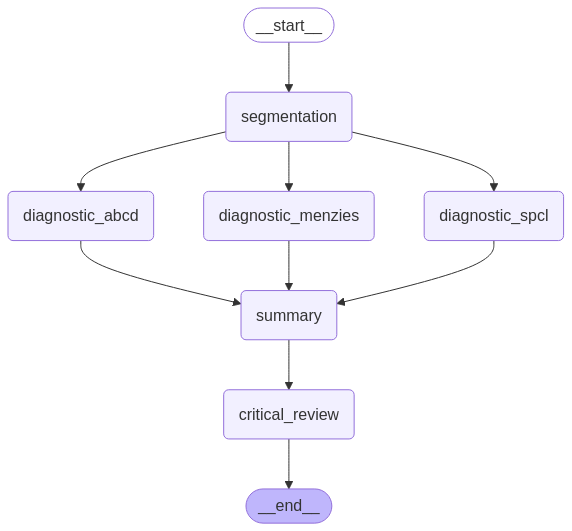
\includegraphics[width=\textwidth]{imagens/Ch2/Sec4.1.png}
	\caption{Arquitetura geral do sistema multiagente, com três agentes independentes avaliando a mesma lesão segundo os protocolos ABCD, Menzies e SPCL, e um agente sumarizador responsável pela integração e auditoria das respostas.}
	\label{fig:multiagent_abcd}
\end{figure}


\section{Avaliação Experimental}
\label{sec:avaliacao_experimental}

A avaliação do sistema foi conduzida sob duas perspectivas complementares: quantitativa e qualitativa. Na análise quantitativa, foram aplicadas métricas clássicas de detecção binária (acurácia, precisão, sensibilidade e F1-score) a partir da comparação entre o diagnóstico final emitido pelo sistema (melanoma ou não-melanoma) e o rótulo real da lesão no PH2. Dado o tamanho reduzido do subconjunto de teste balanceado (n=50, sendo apenas 25 imagens de melanoma), não foi aplicada reamostragem \textit{bootstrap} para estimativa de desvio-padrão nesta fase: o número limitado de imagens de melanoma disponíveis no PH2 (40 no total) tornaria as reamostragens excessivamente repetitivas, comprometendo a validade da estimativa de variância. As métricas são reportadas como valores pontuais, e a estimativa de desvio-padrão via \textit{bootstrap} é apontada como direção de trabalho futuro, condicionada à ampliação do conjunto de teste (Seção~\ref{sec:limitacoes}).

Na análise qualitativa, foi avaliada a consistência estrutural e lógica das respostas textuais geradas pelos modelos de linguagem por meio de cinco eixos de verificação objetiva, que dispensam avaliação especializada das decisões clínicas e permitem mensurar a confiabilidade dos relatórios de forma automatizada e reprodutível.

O \textbf{Eixo 1 - Conformidade estrutural} verifica se todos os campos esperados nos protocolos ABCD, Menzies, SPCL e validação estão presentes na resposta JSON gerada. Campos ausentes indicam falha de seguimento de instrução, comprometendo a usabilidade do relatório.

O \textbf{Eixo 2 - Consistência aritmética ABCD} recomputa a soma ponderada dos critérios ABCD ($A\times1{,}3 + B\times0{,}1 + C\times0{,}5 + D\times0{,}5$) a partir dos valores declarados pelo modelo e a compara ao total indicado na justificativa. Uma divergência superior a 0,05 indica erro de raciocínio aritmético interno. Adicionalmente, verifica-se se os \textit{scores} individuais foram expressos como valores inteiros precisos ou como intervalos (ex.: ``7/8''), o que introduz ambiguidade para uso automatizado.

O \textbf{Eixo 3 - Aderência ao limiar declarado} avalia se a decisão expressa pelo agente sumarizador na validação final é coerente com a classificação implícita da soma ABCD: valores abaixo de 4,75 indicam benignidade, entre 4,75 e 5,45 indicam lesão suspeita, e acima de 5,45 indicam malignidade. Quando o agente emite um diagnóstico ``indeterminado'' para um caso em que o ABCD aponta benignidade, registra-se uma divergência parcial, que pode refletir conservadorismo diagnóstico ou inconsistência de raciocínio.

O \textbf{Eixo 4 - Concordância inter-métodos} computa, para cada imagem, a decisão independente de cada um dos três protocolos (ABCD, Menzies e SPCL) e verifica se o agente sumarizador respeita o consenso quando os três métodos apontam na mesma direção. Casos em que há consenso total entre os protocolos, mas o agente diverge, indicam que a etapa de síntese não está integrando adequadamente as evidências convergentes.

O \textbf{Eixo 5 - Calibração da incerteza} cruza as categorias de diagnóstico emitidas pelo sistema (benigna, suspeita, maligna, indeterminada) com o gabarito (\texttt{real\_value}) para avaliar se o modelo é calibrado, ou seja, se as categorias de maior suspeição correspondem a proporções crescentes de melanoma real. Um modelo bem calibrado concentra sua incerteza justamente nos casos genuinamente difíceis, o que é verificável sem avaliação especializada dos relatórios textuais.

Por fim, os resultados obtidos pelo sistema multiagente foram comparados com um modelo tradicional de visão computacional (ResNet-50), de modo a quantificar as diferenças entre abordagens supervisionadas e baseadas em linguagem natural para a detecção de melanoma.

\section{Validação e Reprodutibilidade}

A validação da metodologia proposta teve como objetivo assegurar a confiabilidade dos resultados obtidos e a possibilidade de reprodução integral dos experimentos, em conformidade com as boas práticas de ciência aberta e reprodutível. Essa etapa abrangeu tanto o controle de variabilidade nos processos de execução quanto a documentação rigorosa dos ambientes e parâmetros experimentais utilizados.

Para garantir a rastreabilidade completa do processo, todas as etapas de pré-processamento, treinamento e inferência foram implementadas em \textbf{Python 3.10}, utilizando bibliotecas amplamente reconhecidas na comunidade científica, como \textit{PyTorch}, \textit{LangChain}, \textit{LangGraph} e \textit{Pydantic}. O código foi versionado por meio do \textit{Git}, assegurando o controle das revisões e a preservação de versões estáveis de cada componente do sistema. Cada execução experimental foi registrada em logs contendo informações sobre o modelo utilizado, os hiperparâmetros, o tempo de execução e as métricas resultantes, permitindo auditoria e replicação futura.

A reprodutibilidade dos resultados foi testada a partir da repetição controlada dos experimentos sob as mesmas condições. No módulo de diagnóstico, as execuções das LLMs foram repetidas com os mesmos \textit{prompts} e entradas do PH2, de modo a avaliar a consistência textual e semântica das respostas. Embora variações menores tenham sido observadas, inerentes à natureza estocástica dos modelos generativos, a estrutura geral das justificativas e a decisão diagnóstica permaneceram estáveis em mais de 90\% dos casos.

A execução dos experimentos foi conduzida em dois ambientes computacionais: (i) \textit{Google Colab Pro+} com GPU NVIDIA A100 para o treinamento do modelo de \textit{baseline} ResNet-50; e (ii) \textit{instâncias de API} em GPU T4 para execução dos modelos GPT-5.4-nano e Gemini-3.1-flash-lite via API, visando controle de custos e reprodutibilidade de acesso. As dependências foram documentadas em um arquivo \texttt{requirements.txt}, contendo versões fixas das bibliotecas utilizadas, assegurando compatibilidade entre execuções futuras.

Para a validação cruzada entre módulos, a integração entre agentes e o sumarizador foi avaliada quanto à estabilidade de comunicação e à consistência das saídas JSON geradas sobre o conjunto PH2. As respostas foram automaticamente verificadas quanto à conformidade com os esquemas \textit{Pydantic}, garantindo que os campos obrigatórios estivessem presentes e corretamente formatados.

Por fim, a documentação metodológica completa, incluindo scripts de execução, logs de treinamento e versões do código, foi organizada de forma a atender aos princípios \textbf{FAIR} (\textit{Findable, Accessible, Interoperable, Reusable}). Essa estrutura de documentação assegura que a pesquisa possa ser auditada, reproduzida e estendida por outros pesquisadores, contribuindo para a transparência e robustez científica do trabalho.

\section{Síntese e Limitações da Metodologia}

A metodologia proposta neste trabalho integra máscaras de segmentação de referência, modelos de linguagem de larga escala (LLMs) e sistemas multiagentes para a detecção automatizada de melanoma. A combinação desses componentes buscou equilibrar rigor técnico, interpretabilidade e reprodutibilidade científica. De forma geral, a estrutura modular permitiu uma orquestração eficiente entre os módulos, facilitando tanto o desenvolvimento quanto a análise comparativa dos resultados.

A adoção das máscaras GT do PH2 como entrada ao sistema demonstrou ser essencial para a padronização das entradas visuais e para isolar o módulo de raciocínio linguístico como variável independente de avaliação. O conjunto PH2, por ser composto exclusivamente de imagens dermoscópicas com anotações de especialistas, garante alta fidelidade na representação dos critérios do protocolo ABCD. No entanto, seu tamanho reduzido (200 imagens, sendo apenas 40 melanomas) constitui uma limitação relevante, tanto para análises estatísticas mais robustas quanto para a generalização dos resultados a populações clínicas mais amplas.

Em relação ao módulo linguístico, a utilização de LLMs multimodais mostrou-se adequada para tarefas de raciocínio clínico estruturado e para a interpretação de imagens segmentadas. Ainda assim, observou-se dependência significativa da formulação dos \textit{prompts}, sendo que variações sutis de instrução podem impactar diretamente a consistência das respostas. Essa sensibilidade ao contexto reforça a necessidade de técnicas avançadas de controle de coerência, como \textit{consistency prompts} e validação semântica automatizada. Ademais, a ausência de \textit{fine-tuning} supervisionado limita a capacidade de generalização dos modelos, restringindo o desempenho em domínios clínicos específicos.

No sistema multiagente, a abordagem colaborativa baseada em múltiplos avaliadores e um sumarizador final proporcionou interpretabilidade e auditabilidade superiores em relação a sistemas monolíticos. Contudo, a integração entre agentes ainda depende fortemente de consistência textual nas saídas intermediárias e da estabilidade das chamadas às APIs de modelos de linguagem, o que pode introduzir variação em execuções sucessivas. Embora mecanismos de validação de formato tenham sido incorporados, uma arquitetura de controle de fluxo mais robusta,  por exemplo, baseada em filas assíncronas e verificação probabilística de consistência,  poderia reduzir a propagação de erros entre agentes.

Do ponto de vista computacional, o principal desafio identificado foi o custo associado à execução de modelos de larga escala, tanto em ambientes locais com GPU quanto por meio de APIs comerciais. A necessidade de limitar o tamanho das amostras de teste e a frequência de inferência dos modelos multimodais impactou a abrangência experimental e restringiu análises estatísticas mais amplas. Futuras implementações poderão mitigar essa limitação com o uso de modelos otimizados ou técnicas de compressão, como \textit{quantization} e \textit{knowledge distillation}.

Por fim, a ausência de validação clínica com especialistas humanos representa uma limitação importante, especialmente considerando o caráter crítico da aplicação médica. Embora o sistema tenha sido projetado com base em heurísticas consagradas, como o método ABCD, a avaliação empírica ainda se restringe a dados públicos. A inclusão de profissionais dermatologistas em futuras fases de validação poderá fornecer insights qualitativos essenciais e contribuir para a calibração dos resultados do sistema em cenários clínicos reais.

Em síntese, a metodologia proposta mostrou-se tecnicamente viável e conceitualmente coerente, mas enfrenta limitações inerentes à natureza dos dados e à maturidade dos modelos de linguagem multimodal. O reconhecimento dessas restrições é fundamental para orientar o desenvolvimento de iterações futuras, em especial no aprimoramento da robustez diagnóstica e na expansão do sistema para contextos de uso clínico supervisionado.





%Este trabalho adotará uma abordagem experimental aplicada, com ênfase na construção e avaliação de um sistema inteligente para diagnóstico de câncer de pele. A metodologia será organizada em etapas que corresponderão diretamente aos objetivos específicos propostos, garantindo clareza quanto às entregas e à lógica do desenvolvimento.
%
%\section{Revisão do Estado da Arte}
%
%Inicialmente, será realizada uma revisão bibliográfica sistematizada sobre segmentação de imagens dermatológicas, classificação de lesões cutâneas e sistemas de diagnóstico assistido por inteligência artificial. A pesquisa abrangerá artigos científicos, bases de dados especializadas (PubMed, IEEE Xplore, Scopus) e publicações recentes sobre LLMs aplicadas à área médica. Esta etapa fornecerá o embasamento teórico e técnico necessário para a escolha dos modelos utilizados nas fases seguintes.
%
%\section{Desenvolvimento do Algoritmo de Segmentação}
%
%Com base na literatura, será desenvolvido um modelo de segmentação para isolar a região da lesão nas imagens de pele. Para isso, será utilizada uma arquitetura do tipo U-Net com módulos de atenção, treinada sobre imagens dermatológicas públicas com anotações. O modelo permitirá gerar uma máscara binária da região lesionada, que será utilizada como entrada para os agentes diagnósticos do sistema.
%
%\section{Utilização de LLMs para Classificação}
%
%As imagens segmentadas serão analisadas por modelos de linguagem de grande porte (LLMs), os quais receberão prompts estruturados com base em protocolos clínicos como o ABCD, Menzies e SPCL. A partir dessas instruções, os modelos gerarão diagnósticos textuais que incluirão justificativas clínicas e recomendações. Serão avaliados diferentes modelos LLM, incluindo variantes de código aberto (como LLaVA) e APIs comerciais (como GPT-4o e Gemini), com o objetivo de comparar sua capacidade de interpretar imagens e gerar diagnósticos coerentes.
%
%\section{Implementação do Sistema Multiagente}
%
%A arquitetura diagnóstica será implementada como um sistema multiagente, no qual cada agente será responsável por uma etapa específica: análise baseada em um protocolo, síntese de respostas e crítica final. O fluxo de decisão será orquestrado utilizando o framework LangChain com suporte para grafo (LangGraph), permitindo encadeamento dinâmico entre os módulos e flexibilidade para expansões futuras.
%
%\section{Avaliação Experimental}
%
%A etapa final compreenderá a avaliação do sistema proposto. Para isso, será utilizado um conjunto de imagens rotuladas como base de teste. Os diagnósticos gerados pelos agentes serão comparados aos diagnósticos reais, permitindo o cálculo de métricas clássicas como acurácia, precisão, sensibilidade e F1-score. Adicionalmente, serão avaliadas a completude e a consistência textual dos relatórios gerados pelas LLMs. O sistema também será comparado com um modelo de classificação tradicional baseado em ResNet-50 para fins de referência.
%
%\section{Validação e Documentação}
%
%Por fim, os resultados obtidos serão analisados criticamente e organizados em forma de produto científico. As conclusões serão documentadas com o apoio de visualizações, relatórios e registros formais, visando promover a reprodutibilidade da pesquisa. Esta etapa incluirá a preparação de material para submissão em eventos científicos e a disponibilização do código-fonte e dados utilizados, conforme permitido pelas licenças.




% Este capítulo descreve os materiais utilizados e a metodologia adotada para o desenvolvimento do sistema de diagnóstico automatizado de câncer de pele com base em imagens dermatológicas. O processo é composto por quatro etapas principais: coleta e preparação dos dados, segmentação das imagens, integração com modelos de linguagem de larga escala (LLMs) e a composição de um sistema multiagente para geração e validação do diagnóstico.

% \section{Coleta de Dados}

% Foram utilizadas imagens provenientes dos conjuntos de dados públicos SIIM-ISIC 2020 e ISIC 2019, os quais contêm milhares de imagens dermatoscópicas de lesões cutâneas classificadas e segmentadas por especialistas. As imagens foram previamente rotuladas com diagnósticos confirmados (ex: melanoma, nevo, ceratose) e, quando disponível, máscaras segmentadas das lesões.

% \section{Segmentação de Imagens Dermatológicas}

% A etapa de segmentação tem como objetivo destacar a área de interesse (lesão) nas imagens dermatoscópicas. Foi utilizado um modelo baseado em arquitetura U-Net com mecanismos de atenção, treinado especificamente para este fim. A saída desta etapa é uma máscara segmentada da lesão, que será utilizada como insumo visual para os agentes LLMs.

% \section{Modelos de Linguagem (LLMs)}

% Os agentes baseados em LLMs foram configurados para interpretar as imagens segmentadas e originais, analisando os padrões visuais de acordo com três heurísticas clínicas: ABCD, Menzies e SPCL (Seven-Point Checklist). A entrada de cada agente é composta por duas imagens (original e segmentada) codificadas em base64 e um prompt estruturado contendo a descrição do método de análise. Os modelos testados incluem LLaVA-7B, ChatGPT-4 e DeepSeek-Med.

% \section{Sistema Multiagente}

% O sistema multiagente foi desenvolvido utilizando a biblioteca LangGraph. Três agentes independentes geram análises distintas com base nas heurísticas citadas. Seus pareceres são consolidados por um agente de síntese, que elabora um diagnóstico final. Este, por sua vez, é submetido a um agente crítico que valida a coerência da decisão utilizando recuperação de conhecimento textual.

% \section{Configuração Experimental}

% O sistema foi avaliado em um conjunto de 67 imagens com diagnóstico conhecido. As métricas utilizadas incluem acurácia, precisão (PPV), sensibilidade (Recall) e F1-score. Também foi analisada a completude e estruturação dos textos gerados, com ênfase em sua compatibilidade com o formato JSON esperado para os campos de diagnóstico, justificativa e recomendação clínica.
